% alt + shift + 1
% make projname.pdf
% wordcount: detex writeup.tex | wc -w

\documentclass[12pt]{article}
%------------------------Dimensions----------------------------

\topmargin=0.0in
\oddsidemargin=0.0in           % 1in margins at left and right
\evensidemargin=0in
\textwidth=6.5in               % US paper is 8.5in wide
\marginparwidth=0.5in

\headheight=0pt                % 1in margins at top and bottom
\headsep=0pt
\topmargin=0in
\textheight=9.0in              % US paper is 11.0in high

%adjustments...
\addtolength{\topmargin}{-0.5in}
\addtolength{\textheight}{1.0in}
\addtolength{\textwidth}{0.5in}
\addtolength{\oddsidemargin}{-0.25in}
\addtolength{\evensidemargin}{-0.25in}
                       
\pagestyle{empty}

%------------------------Packages----------------------------
\usepackage{textcomp}
\usepackage{longtable}
\usepackage{setspace}
\usepackage{amsmath,amssymb,amsthm}
\usepackage{graphicx}
\usepackage{epsfig}
\usepackage{subfig}
\usepackage[paperwidth=8.5in,paperheight=11in,margin=0.98in]{geometry}
\usepackage{listings,float}
\usepackage{color}
\usepackage{array}
\usepackage{cancel}

%------------------------Commands----------------------------
\newcommand{\be}{\begin{enumerate}}
\newcommand{\ee}{\end{enumerate}}
\newcommand{\bi}{\begin{itemize}}
\newcommand{\ei}{\end{itemize}}
\newcommand{\bv} {{\bf v}}
\newcommand{\bD} {{\bf D}}

\definecolor{listinggray}{gray}{0.9}
\definecolor{lbcolor}{rgb}{0.9,0.9,0.9}
\lstset{
	tabsize=4,
	rulecolor=,
	language=matlab,
	keywords={break,case,catch,continue,else,elseif,end,for,function,
      global,if,otherwise,persistent,return,switch,try,while},
        basicstyle=\footnotesize\ttfamily,
        upquote=true,
        aboveskip={1.5\baselineskip},
        columns=fixed,
        showstringspaces=false,
        extendedchars=true,
        breaklines=true,
        prebreak = \raisebox{0ex}[0ex][0ex]{\ensuremath{\hookleftarrow}},
        frame=single,
        showtabs=false,
        showspaces=false,
        showstringspaces=false,
        identifierstyle=\ttfamily,
        keywordstyle=\color[rgb]{0,0,1},
        commentstyle=\color[rgb]{0.133,0.545,0.133},
        stringstyle=\color[rgb]{0.627,0.126,0.941},
}

\captionsetup{width=.75\textwidth} 

\begin{document}
\pagestyle{plain} %pagenumbers
\title{CSCI 4/5576: The Random Logistic Map}
\date{December 17, 2014}
\author{Amy Le (5576)\\Long Tat (4576)\\Emily Bertelson (4576)\\Kristina Entzel (4576)}
\maketitle
\section{Abstract}
The purpose of this investigation was to explore and simulate a
spatially random logistic map using a dynamic load balancer on Janus, the CU
supercomputer. The recursive nature of the map prevents the individual
fixed point iterations from being parallelized, but a set of
iterations maybe load balanced over many cores. The original simulation was written in serial code in
MATLAB. Our solution has modified the original version for efficiency,
speed, and scalability. We implemented our simulation in C++ and present our
results in terms of a histogram of observed periodic orbits and a
bifurcation diagram. Single core optimization techniques,
such as SIMD loop vectorization and function inlining, as well as
using a dynamic load balancer for more efficient work distribution
were applied. The HDF5 file format was used to store the simulation results in a better archival format. The benchmarking (weak scaling study) results imply the best
speedup and efficiency is gained when invoking the load balancer on
one node (12 cores), although we tested our simulation over 16 nodes
(192 cores). Improvements to this project include optimizing the
post-simulation data processing. 
\section{Introduction}
\hspace{5mm}The Logistic map is a quadratic recursive equation on the domain
[0,1]. It is a popularly studied topic in nonlinear dynamics and has
applications in population modeling. There is one parameter in the
expression, $r$, which can take any value in the range [0,4]. 
\begin{equation*}
x_{n+1} = rx_n(1-x_n)
\end{equation*}
For values of $r \in [3.5,4]$, the system experiences the onset of
chaos. Between $r \in [0,3.5]$, we observe stable periodic orbits.
\begin{figure}[H]
	\begin{center}
		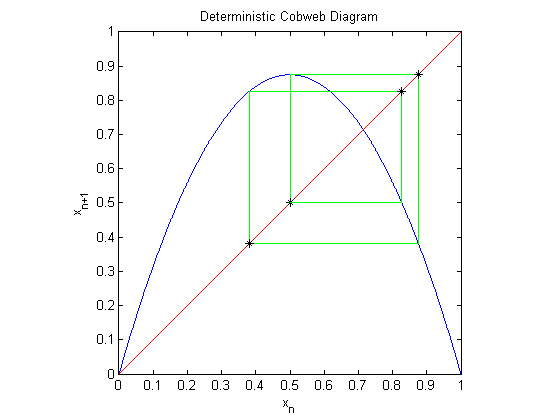
\includegraphics[scale=0.7]{det_cobweb}
\caption{Deterministic Logistic Map (blue) for $r=3.2$. There is a stable period
4 orbit. The order of the period is calculated by counting the number
of crossings (green) on the line $x_{n+1}=x_n$ (red).}
	\end{center}
\end{figure}
\begin{figure}[H]
	\begin{center}
		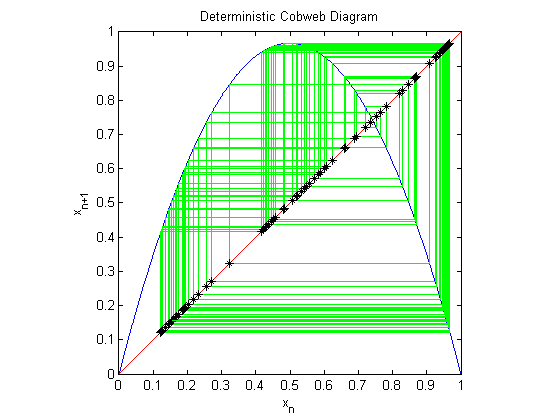
\includegraphics[scale=0.7]{chaos}
\caption{Deterministic Logistic Map (blue) for $r=3.8$. There is a no stable orbit.}
	\end{center}
\end{figure}
There are two ways to vary the deterministic map. We can simulate the
parameter $r$ as a function of time or space. The existing literature
explore the notion of randomness in time, so we explore $r$ as a
function of space \cite{athreya}.

The following equation is the fixed point iteration that the code
completes, where $R(x)$ is calculated by manipulating a random number generator.
\begin{equation*}
x_{n+1} = R(x_n)x_n(1-x_n)
\end{equation*}
The exact details of how to calculate $R(x)$ are outlined below.
\begin{align*}
\begin{split}
\ln(R(x)) &= \xi(x)\\
\xi(x) &= \ln(r) + 2\sum^N_{n=1}a_n\cos(2\pi nx)-b_n\sin(2\pi nx)\\
a_n,b_n &\sim Unif(-M_n,M_n)\\
M_n &= \sqrt{1.5S_n}\\
S_n &= \alpha e^{-L|n|}\\
\alpha &= \sigma^2 \tanh(L/2)\\
\sigma &< \ln(4/r)\frac{\tanh(L/4)}{\sqrt{1.5\tanh(L/2)}}
\end{split}
\end{align*}
Where $L \in (0,1)$ represents the correlation length (and is fixed
for each simulation) and $r \in [0,4]$ is also fixed for each
simulation. 
\begin{figure}[H]
	\begin{center}
		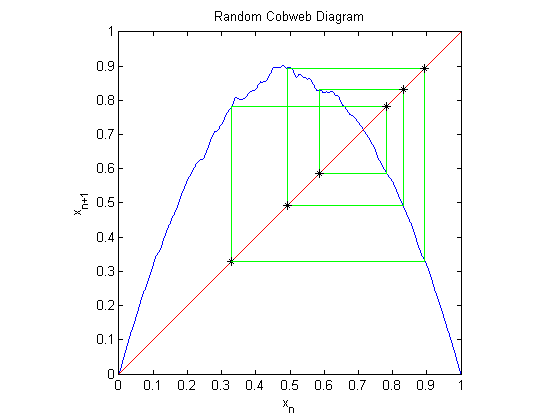
\includegraphics[scale=0.7]{rand_cobweb}
\caption{One instance of a random logistic map (blue). The map has
  converged to a stable period 6 orbit (green). Notice the
  ``wiggliness'' in the parabola shape.}
	\end{center}
\end{figure}
Other instances of the random map would vary from this realization,
due to the random nature of the map. 
\begin{figure}[H]
	\begin{center}
		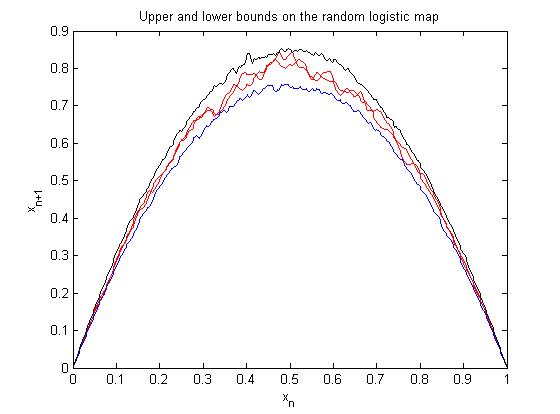
\includegraphics[scale=0.7]{envelope}
\caption{A coarse demonstration of the upper (black) and lower (blue) bounds of the
  random logistic map. Sample realizations are shown in red.}
	\end{center}
\end{figure}
Since the map can take on a range of values for any given position in
space, it would be useful to characterize some of its properties. In particular, we will be studying the stability of the map,
which includes locating fixed points and generating bifurcation
diagrams. The two main goals are:
\be
\item Find the expected number of order $p$ periodic orbits for a
  the random map ($p = 1, 2, 3, ...$)
\be
\item For an initial starting value $x_0 \in [0,1]$ and a specific
  random function $R_0(x)$, iterate until you
  find the fixed point(s), $x_i^*$ associated with $R_0(x)$. 
\item Classify the fixed points in terms of a period $p$ orbit. 
\item Each processor should take a different initial $x_0$ and report
  whether the initial condition led to finding a unique stable orbit  
\bi
\item The processors should be properly load balanced.
\item As each processor finishes its work, it will write its results
  to an HDF5 file (parallel i/o)
\ei
\item Repeat the above steps for a large number of different random
  maps $R_i(x)$, $i = 0, 1, 2,... \bar{N}$ in order to find the expected
  number of order $p$ periodic orbits for the random map.
\ee
\item Create a set valued bifurcation diagram \cite{lamb}
\be
\item For many values of $r \in [0,4]
$, and a fixed random function
  $R_0(x)$, plot the locations of the periodic orbits as a function of
  $r$. A period $p$ orbit will have $p$ corresponding $x$ values as
  its orbit locations (e.g. a period 1 orbit will have 1 fixed point,
  a period 2 orbit will have 2 fixed points, and so on). 
\bi
\item Use a HDF5 file to store the simulation data and as a source to generate
  bifurcation diagrams
\ei
\ee
\ee
As the map has an element of randomness to it, many
simulations (a large $\bar{N}$) would be required for statistical analysis. 
\section{Method}
The general progression of the project is outlined below:
\be
\item Convert the Matlab code to C++
\item Confirm the C++ versions of the code that we each produce work
  together correctly by comparing to the serial version
\item Invoke the load balancer to assign an initial condition to each
  fixed point iteration 
\item Benchmark: strong scaling study (speedup and efficiency)
\ee
\noindent The table below summarizes how we have subdivided the project among
ourselves. 
\begin{figure}[H]
	\begin{center}
		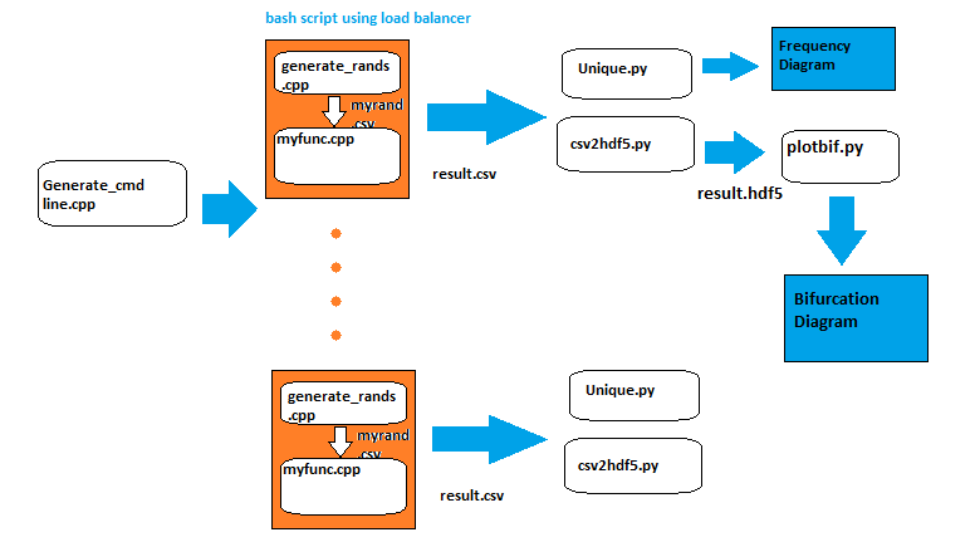
\includegraphics[scale=0.5]{workflow}
\caption{Workflow}
	\end{center}
\end{figure}
\subsection{Single Core Optimization}
Optimizations implemented in the code conversion:
\bi
\item Preferential use of the  multiply and add operators where possible, since
they less expensive than subtract and divide operators
\item I used a reduction on the loop that computes the Fourier Series
  in order to take advantage of the data parallelism with SIMD
\item Loop structure was reorganized to take advantage of C++ being row-oriented
\item I used inlining in the C++ code to reduce the number of function calls
\item The lack of a built in uniform random number generator that generates a random
double between two doubles made me create a psudeo random number
implementation with the use of \texttt{rand} and \texttt{srand}.
\lstinputlisting{rand_ex.m}
\ei
\subsection{Load Balancer}
\begin{figure}[H]
	\begin{center}
		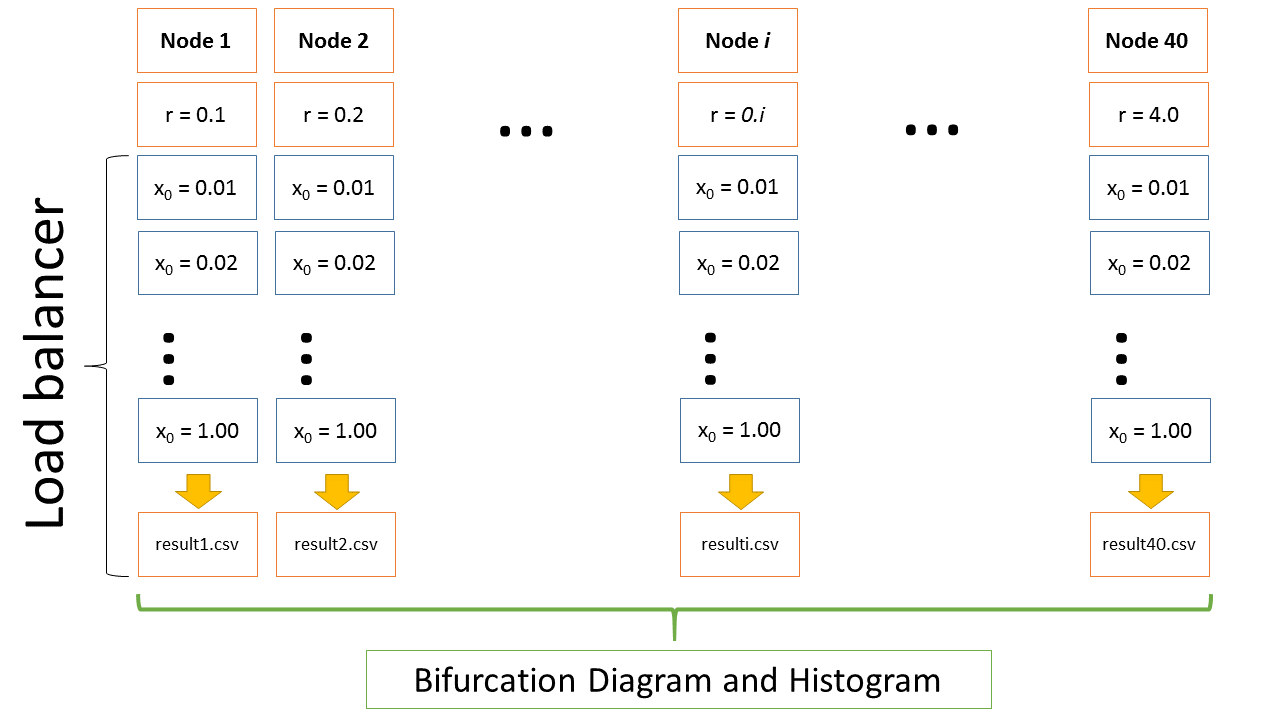
\includegraphics[scale=0.4]{load_balancer}
\caption{Load balancer.}
	\end{center}
\end{figure}
We researched types of load balancers \cite{olivier}. We found there
are many strategies for load balancing \cite{dlb}.
\subsection{HDF5}
A structure for the file has been devised:
\begin{tabbing}
	\hspace{5mm} group ``$r$'' \\
		\hspace{10mm} group ``$L$'' \\
		\hspace{15mm} group ``$p=1$'' \\
				\hspace{20mm} dataset \\
					\hspace{25mm} $ (x_{1})$ \\
					\hspace{25mm} $ (x_{2})$ \\
					\hspace{25mm} $ (x_{3})$ \\
					\hspace{25mm} ... \\	
			\hspace{15mm} group ``$p=2$'' \\
				\hspace{20mm} dataset \\
					\hspace{25mm}                           $(x_{11},x_{12})$ \\
					\hspace{25mm} $(x_{21},x_{22})$ \\
					\hspace{25mm} ... \\
\end{tabbing}

\begin{tabbing}
  \hspace{5mm} group ``$L$'' \\
  \hspace{10mm} dataset \\
  \hspace{15mm} $ (x_{1}, r, p=1)$ \\
  \hspace{15mm} $ (x_{1},x_2, r, p=2)$ \\
  \hspace{15mm} ... \\
  \hspace{15mm} $ (x_{1},x_2,...x_k, r, p=k)$ \\
\end{tabbing}

From there, HDF5 compatibility will be implemented in code where
relevant \cite{folk} \cite{UserGuide}. 
\section{Results}
\begin{figure}[H]
	\begin{center}
		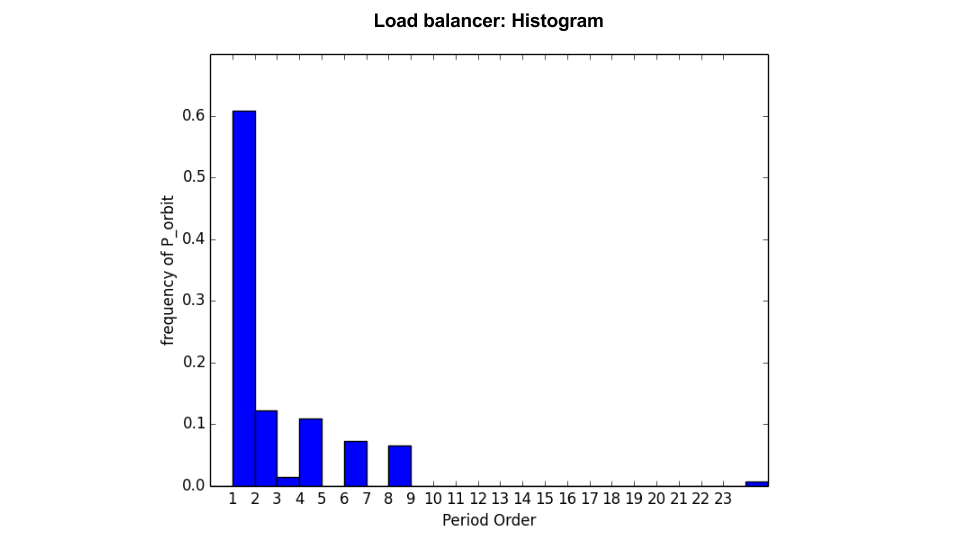
\includegraphics[scale=0.4]{hist}
\caption{load balanced histogram}
	\end{center}
\end{figure}
\begin{figure}[H]
	\begin{center}
		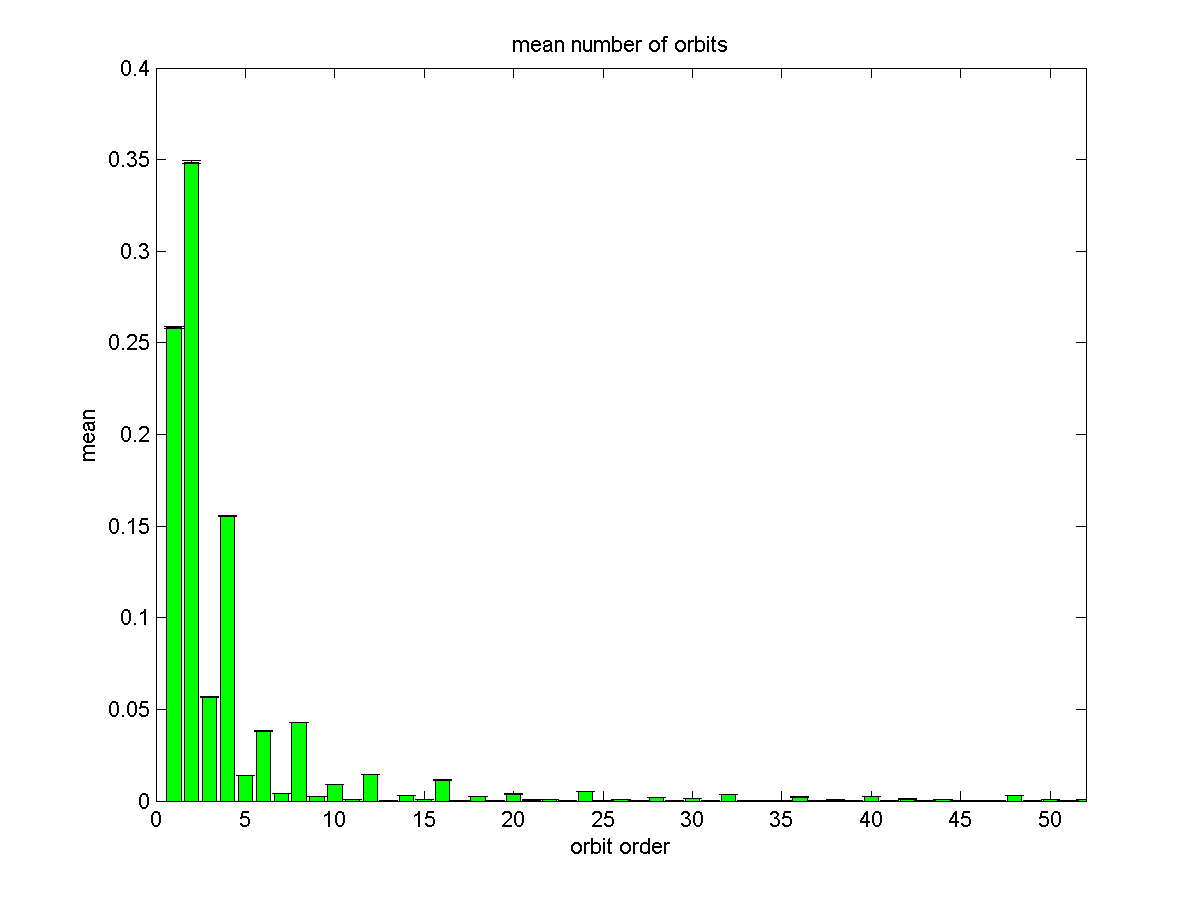
\includegraphics[scale=0.5]{serial_hist}
\caption{serial histogram}
	\end{center}
\end{figure}

\begin{figure}[H]
	\begin{center}
		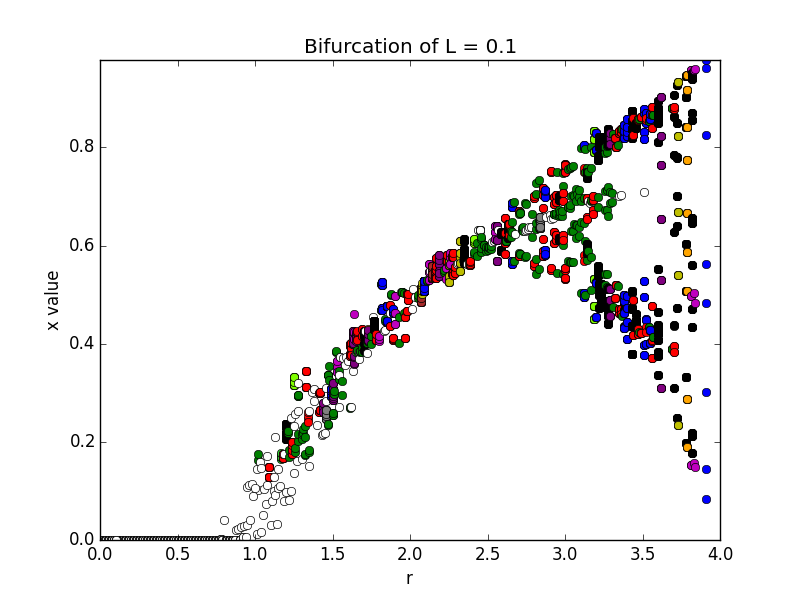
\includegraphics[scale=0.5]{Bifurcation_L1}
\caption{Bifurcation with $L=0.1$}
	\end{center}
\end{figure}
\begin{figure}[H]
	\begin{center}
		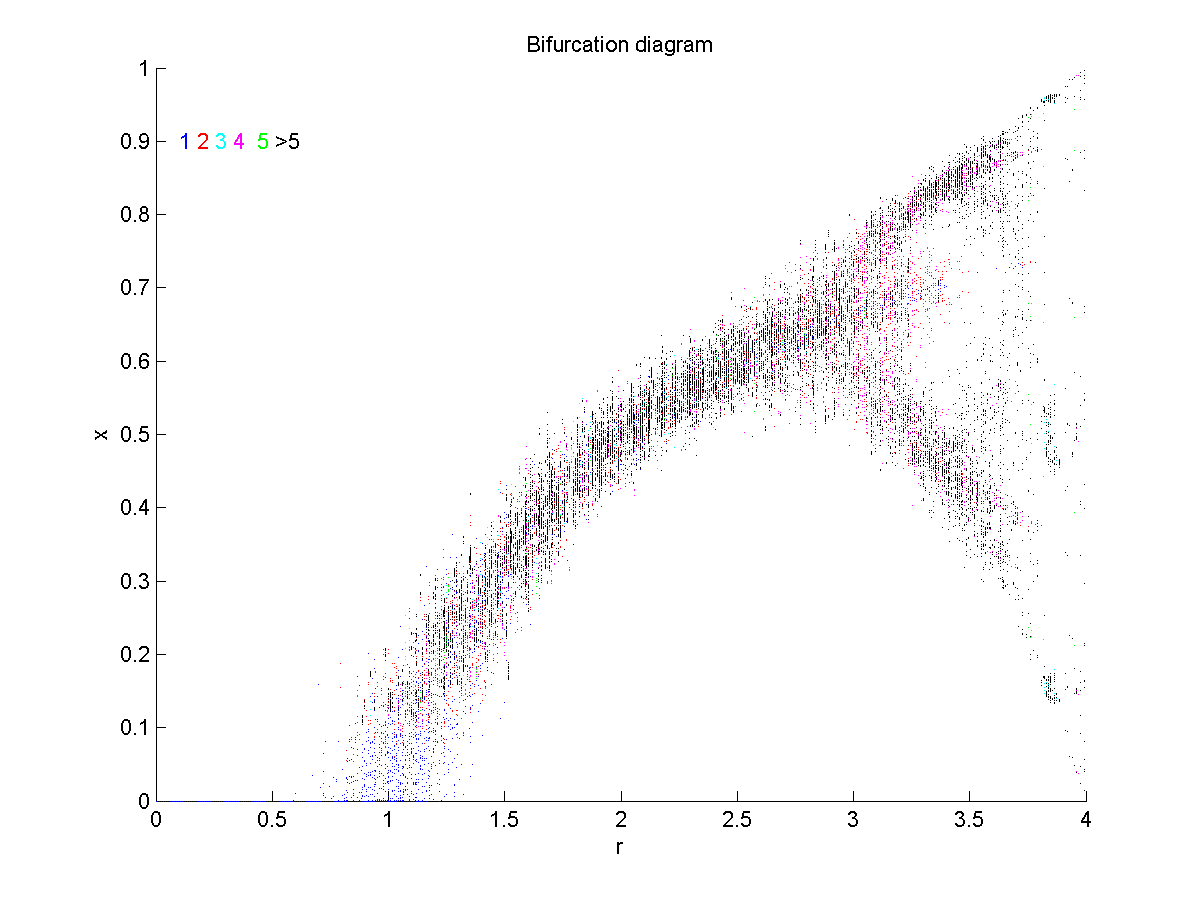
\includegraphics[scale=0.5]{bif}
\caption{serial bifurcation}
	\end{center}
\end{figure}

\begin{figure}[H]
	\begin{center}
		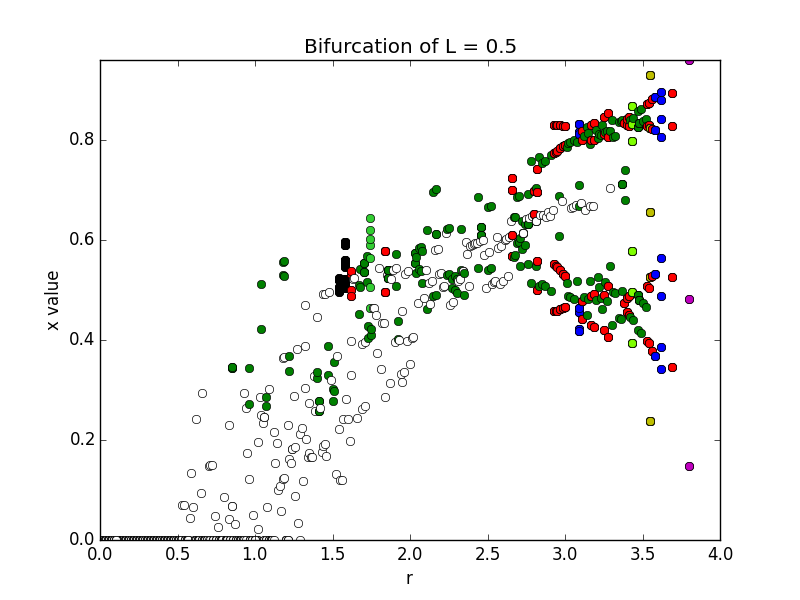
\includegraphics[scale=0.5]{Bifurcation_L5}
\caption{Bifurcation with $L=0.5$}
	\end{center}
\end{figure}
\begin{figure}[H]
	\begin{center}
		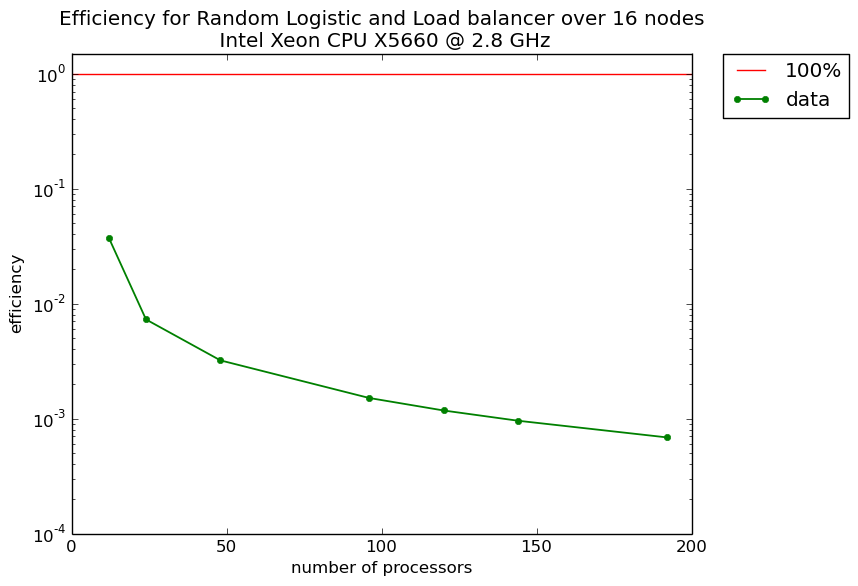
\includegraphics[scale=0.5]{efficiency_random_logistic}
\caption{Efficiency}
	\end{center}
\end{figure}
\begin{figure}[H]
	\begin{center}
		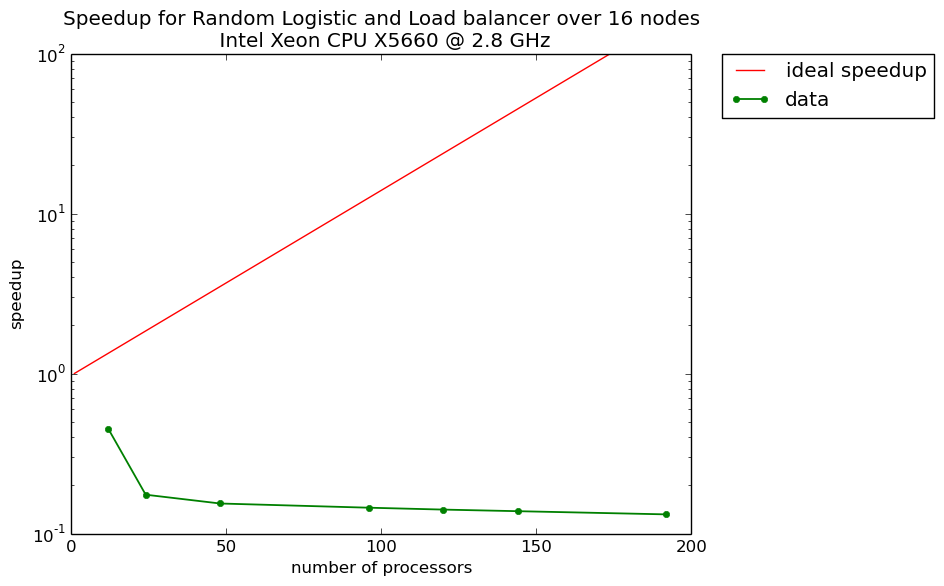
\includegraphics[scale=0.5]{speedup_random_logistic}
\caption{Efficiency}
	\end{center}
\end{figure}

\section{Conclusion}
\subsection{Future Work}

\bibliographystyle{plain}
\bibliography{annot}

\end{document}
